\documentclass[12pt,oneside,a4paper]{book}
\usepackage[utf8]{inputenc}
\usepackage[T1]{fontenc}
\usepackage[english]{babel}

\usepackage{setspace}

\usepackage[margin=2.54cm]{geometry}
\usepackage[spanish]{nomencl}
\renewcommand{\nomname}{Lista de abreviaturas}
\makenomenclature
\usepackage{etoolbox}
\usepackage{mathptmx}
\usepackage{fancyhdr}
\usepackage{amsmath,amsfonts,amssymb} 
\usepackage{caption} 
\DeclareCaptionLabelSeparator*{spaced}{\\[1.5ex]}
\captionsetup[table]{textfont=it,format=plain,justification=justified,singlelinecheck=false,labelsep=spaced,skip=0pt, labelfont=bf}
%\captionsetup[figure]{labelsep=period,labelfont=it,justification=justified,
%	singlelinecheck=false,font=doublespacing}
\captionsetup[figure]{textfont=it,format=plain,justification=justified,singlelinecheck=false,labelsep=spaced,skip=0pt, labelfont=bf}

\newcommand{\sep}{\vspace{0.3cm}}

\usepackage{setspace}
\usepackage{graphicx} 
\usepackage{csquotes}
\usepackage{changepage}
\usepackage{subcaption}	% Para subfiguras
\usepackage{makeidx}
\usepackage{multirow}
\usepackage{array} 
\usepackage{float}
\usepackage{pdflscape} % Página horizontal
\usepackage{lscape} % Hoja horizontal
\usepackage{pdfpages}
\usepackage{wallpaper}
\usepackage{acronym}
\usepackage{tikz}% Para desarrollar funciones
\usepackage{url} % Para insertar url sin problemas
\usepackage{xcolor} % Para texto con diferente colores
\usepackage{tablefootnote} 
\usepackage{lipsum}
\usepackage{enumitem}
\usepackage{marginnote}
\usepackage{indentfirst}
% \usepackage{natbib}

%\usepackage[hidelinks]{hyperref}
\usepackage{hyperref}
\hypersetup{
    colorlinks=true,
    %linkcolor=blue,
    %filecolor=magenta,      
    urlcolor=red,
    citecolor=blue,
    %pdftitle={Overleaf Example},
    %pdfpagemode=FullScreen,
    }

\definecolor{marron}{RGB}{128,64, 0}
\definecolor{naranja}{RGB}{255,70, 0}

\newcommand{\propuesta}[1]{  
  \textcolor{red}{#1}
}
\newcommand{\metodo}[1]{
  \textcolor{blue}{#1}
}
\newcommand{\resultados}[1]{
  \textcolor{marron}{#1}
}
\newcommand{\conclusiones}[1]{
  \textcolor{naranja}{#1}
}





%\setlength{\leftmargini}{1em}

\usepackage{appendix}
\newcommand\listappendixname{Índice de anexos}
\newcommand\appcaption[1]{%
  \addcontentsline{app}{section}{#1}}
\makeatletter
\newcommand\listofappendices{%
% \setlength{\parskip}{0.2em} 
  \chapter*{\listappendixname}\@starttoc{app}}
\makeatother

\usepackage{titlesec}
\titleformat{\chapter}[block]
{\vspace{-0.56cm}
{\fontsize{14pt}{ \baselineskip}\selectfont}\bfseries\centering}
{\thechapter}{1em}{\vspace{-1.3cm}}
\titleformat{\section}[block]
{\vspace{0cm}
{\fontsize{12pt}{ \baselineskip}\selectfont}\bfseries}
{\thesection}{1em}{\vspace{-0.4cm}}
\titleformat{\subsection}[block]
{\vspace{-0.6cm}
{\fontsize{12pt}{ \baselineskip}\selectfont}\bfseries}
{\thesubsection}{1em}{\vspace{-0.4cm}}
\titleformat{\subsubsection}[block]
{\vspace{-0.6cm}
{\fontsize{12pt}{ \baselineskip}\selectfont}\bfseries}
{\thesubsubsection}{1em}{\vspace{-0.3cm}}

\renewcommand{\thesection}{\arabic{chapter}.\arabic{section}}
\renewcommand{\thechapter}{\Roman{chapter}.}
\AtBeginDocument{
\renewcommand{\contentsname}{Índice general}
\renewcommand{\listtablename}{Índice de tablas}
\renewcommand{\listfigurename}{Índice de figuras}
% \renewcommand{\contentsname}{Lista de Contenidos}
% \renewcommand{\refname}{VIII. REFERENCIAS}
\renewcommand{\figurename}{Figura}
\renewcommand{\tablename}{Tabla}
\renewcommand{\thefigure}{\arabic{chapter}.\arabic{figure}}
\renewcommand{\thetable}{\arabic{chapter}.\arabic{table}}
\renewcommand{\theequation}{\arabic{chapter}.\arabic{equation}}
} % Poner nombre a la Tabla
\setcounter{secnumdepth}{6}% para añadir párrafos y subpárrafos
\setcounter{tocdepth}{5}%para que salgan en la tabla de contenidos los párrafos y subpárrafos

\usepackage[natbib=true, backend=biber, style=apa, citestyle=apa, sorting = nyt]{biblatex}
\addbibresource{References/References.bib}

\usepackage[flushleft]{threeparttable}
\usepackage{booktabs}
\renewcommand{\headrulewidth}{0pt}
\renewcommand{\baselinestretch}{1.5}

\doublespacing

\begin{document}
\frontmatter


\newgeometry{top=2.5cm, bottom= 2.5cm, right=2.5cm, left=2.5cm}
\begin{titlepage}
\centering
 {\fontsize{16pt}{ \baselineskip}\selectfont \textbf{UNIVERSIDAD NACIONAL FEDERICO VILLARREAL}}\\[0.2cm]
 {\fontsize{14pt}{ \baselineskip}\selectfont \textbf{FACULTAD DE CIENCIAS NATURALES Y MATEMÁTICA}}\\[0.3cm]
\begin{figure}[htb]
\centering

\includegraphics[width=3.5cm]{Cover/UNFV.png}
\end{figure}
\vspace{0.2cm}
\rule{132mm}{0.25mm}\\
{\fontsize{14pt}{ \baselineskip}\selectfont \textbf{Implementación de una red neuronal para la solución de la ecuación de onda en dos dimensiones}}
\rule{132mm}{0.25mm}\\
{\fontsize{12pt}{ \baselineskip}\selectfont {Tesis para optar el Título Profesional de Licenciado en Física}}\\[0.3cm]

{\fontsize{12pt}{ \baselineskip}\selectfont {AUTOR\\ David Brandon Zevallos Garay
}}\\[0.1cm]

{\fontsize{12pt}{ \baselineskip}\selectfont {ASESOR\\
David Brandon Zevallos Garay
}}\\[0.1cm]

% {\fontsize{12pt}{ \baselineskip}\selectfont {JURADOS\\
% David Brandon Zevallos Garay
% }}\\[0.1cm]

% \large{\textbf{LIMA-PERÚ \\ 2020}}
\vfill
%\vspace*{fill}
{\fontsize{12pt}{ \baselineskip}\selectfont \textbf{LIMA - PERÚ}}\\[0.2cm]
{\fontsize{12pt}{ \baselineskip}\selectfont \textbf{2022}}
%\rule{132mm}{0.25mm}\\
%{\small \textbf{La UNALM es titular de los derechos patrimoniales de la presente investigación\\ (Art.24 - Reglamento de propiedad intelectual)}}
\end{titlepage}
\restoregeometry
% \newgeometry{margin= 2.5cm}

\pagenumbering{roman}

%\begin{center}
\thispagestyle{empty}
 {\fontsize{18pt}{ \baselineskip}\selectfont \textbf{UNIVERSIDAD NACIONAL AGRARIA LA MOLINA}}\\[0.25cm]
 {\fontsize{16pt}{ \baselineskip}\selectfont \textbf{FACULTAD DE INGENIERÍA AGRÍCOLA}}\\[1cm]
 {\fontsize{16pt}{ \baselineskip}\selectfont \textbf{``TÍTULO''}}\\[0.5cm]
 {\fontsize{16pt}{ \baselineskip}\selectfont TESIS PARA OPTAR EL TÍTULO PROFESIONAL DE:}\\[0.5cm]
 {\fontsize{16pt}{ \baselineskip}\selectfont\textbf{INGENIERO AGRÍCOLA}}\\[0.5cm]
 {\fontsize{14pt}{ \baselineskip}\selectfont Presentado por:} \\[0.5cm]
 {\fontsize{16pt}{ \baselineskip}\selectfont \textbf{BACH. ...}}\\[0.5cm]
 {\fontsize{14pt}{ \baselineskip}\selectfont Sustentado y aprobado por el siguiente jurado:}\\[1cm]
\begin{minipage}{\linewidth}
\centering
\singlespacing
\begin{tabular}{cc}
\hrulefill & \hrulefill \\
 {\fontsize{10pt}{ \baselineskip}\selectfont{Dr. ...}} &  {\fontsize{10pt}{ \baselineskip}\selectfont Dr. Mg. Sc. Ing. ...} \\
\small{\textbf{Presidente}} & \small{\textbf{Asesora}}
\end{tabular}\\[1cm]
\begin{tabular}{cc}
\hrulefill & \hrulefill \\
{\fontsize{10pt}{ \baselineskip}\selectfont{Mg. Sc. ...}} & {\fontsize{10pt}{ \baselineskip}\selectfont{Mg. Sc. ...}} \\
\small{\textbf{Miembro}} & \small{\textbf{Miembro}}
\end{tabular}\\[1cm]
\begin{tabular}{c}
\hrulefill \\
{\fontsize{10pt}{ \baselineskip}\selectfont{Ing. ...}} \\
\small{\textbf{Co-Asesor}} 
\end{tabular}
\end{minipage}
\vfill
{\fontsize{14pt}{ \baselineskip}\selectfont \textbf{LIMA - PERÚ}}\\[0.5cm]
{\fontsize{14pt}{ \baselineskip}\selectfont \textbf{2021}}
\singlespacing
\end{center}
%\addcontentsline{toc}{chapter}{\textbf{PORTADA}}

% \newgeometry{top=7cm, bottom= 4cm, right=2.5cm, left=6cm}
\chapter*{\hfill DEDICATORIA}
\thispagestyle{empty}
\doublespacing
\begin{flushright}
\textit{Dedicado a toda mi familia, en especial a mis padres, Miriam y Teodoro, por nunca haberme quitado la curiosidad. También a mi hermana, por escucharme a pesar de no entenderme.}
\end{flushright}


%\addcontentsline{toc}{chapter}{\textbf{DEDICATORIA}}
% \restoregeometry
% \chapter*{\flushright AGRADECIMIENTO}
\doublespacing
\begin{flushright}
       A mis profesores, compañeros, amigos, padres,...
\end{flushright}

%\addcontentsline{toc}{chapter}{\textbf{AGRADECIMIENTO}}

\doublespacing
\tableofcontents

%\addcontentsline{toc}{chapter}{\textbf{ÍNDICE GENERAL}}
%\pagestyle{fancy}
%\fancyhf{}
%\fancyfoot[c]{\thepage}

\listoftables
%\addcontentsline{toc}{chapter}{\textbf{ÍNDICE DE TABLAS}}

\listoffigures
%\addcontentsline{toc}{chapter}{\textbf{ÍNDICE DE FIGURAS}}

\listofappendices
%\addcontentsline{toc}{chapter}{\textbf{ÍNDICE DE ANEXOS}}

\doublespacing
\setlength{\parskip}{1em}
\setlength{\parindent}{0cm}
% \clearpage
\onehalfspacing
\mbox{}

\nomenclature{RNs}{Redes Neuronales}
\nomenclature{RN}{Red Neuronal}
\nomenclature{EDO}{Ecuaciones Diferenciales Ordinarias}
\nomenclature{EDP}{Ecuaciones Diferenciales Parciales}
\nomenclature{PINNs}{Physics-Informed Neural Networks}
\nomenclature{RNA}{Redes Neuronales Artificiales}
\nomenclature{ED}{Ecuaciones Diferenciales}
\nomenclature{IA}{Inteligencia Artificial}
% \nomenclature{SEBAL}{Algoritmo de balance de energía superficial para tierra}
% \nomenclature{SEB}{Componentes del balance de energía}
% \nomenclature{METRIC}{Mapeo de la evapotranspiración a alta resolución con calibración internalizada}
% \nomenclature{METRIC-HR}{METRIC de alta resolución}
% \nomenclature{DTD}{Diferencia de temperatura dual}
% \nomenclature{ANN}{Neuronales artificiales}
% \nomenclature{ML}{Machine learning}
% \nomenclature{DL}{Deep learning}
% \nomenclature{RSEB}{Balance energético con información de teledetección}
% \nomenclature{IAF}{Índice de área foliar}
% \nomenclature{SAVI}{Índice de vegetación ajustado al suelo}
% \nomenclature{NDVI}{Índice de Vegetación de Diferencia Normalizada}
% \nomenclature{BRDF}{Función de distribución de reflectancia bidireccional}
% \nomenclature{NDVIc}{Índice de Vegetación de Diferencia Normalizada para el canopy}
% \nomenclature{NDVIss}{Índice de Vegetación de Diferencia Normalizada para el suelo}
% \nomenclature{TSEB}{Balance de energía de dos fuentes}
% \nomenclature{STSEB}{Salance energético simplificado existente de dos fuentes}
% \nomenclature{ET}{Evapotranspiración}
% \nomenclature{ET}{Evapotranspiración}
% \nomenclature{ETo}{Evapotranspiración de referencia}
% \nomenclature{Etc}{Evapotranspiración real o del cultivo}
% \nomenclature{G}{Flujo de calor del suelo}
% \nomenclature{H}{Flujo de calor sensible}
% \nomenclature{$\mathrm{R_{n}}$}{Radiación neta}
% \nomenclature{$R_{s}$}{Radiación de onda corta entrante}
% \nomenclature{$R_{l}$}{Radiación de onda larga entrante}
% \nomenclature{LE}{Flujo de calor latente}
% \nomenclature{$LE_{v}$}{Transpiración del dosel}
% \nomenclature{$LE_{s}$}{Evaporación del agua del suelo}

\printnomenclature[1in]

%\doublespacing
%\setlength{\parindent}{0cm}
%\setlength{\parskip}{1em} 
%\chapter*{RESUMEN}
\lipsum[1]

\lipsum[2]\\\vspace{1em}

\textbf{Palabras claves:} Zonificación Agroecológica, Duraznero, Proceso Analítico Jerarquizado, Sistemas de Información Geográfica, San Pablo de Pillao, Sequías.
%\addcontentsline{toc}{chapter}{\textbf{RESUMEN}}

%\chapter*{ABSTRACT}

\lipsum[1]

\lipsum[2]\\\vspace{1em}

\textbf{Key Words:} Agroecological Zoning, Peach, Hierarchical Analytical Process, Geographic Information Systems, San Pablo de Pillao, Droughts.
%\addcontentsline{toc}{chapter}{\textbf{ABSTRACT}}

\newpage
\doublespacing
\mainmatter
\pagestyle{fancy}
\fancyhf{}
\rhead[c]{\thepage}

%\setlength{\parskip}{\baselineskip} 
\setlength{\parindent}{1.27cm}
\setlength{\parskip}{1.5em}

\doublespacing

\chapter{Introducción}

\thispagestyle{empty}
% 
% 
% Descripción y formulación del problema
% 
% 
\section{Descripción y formulación del problema}
Las redes neuronales se usan como buenos aproximadores de funciones, pueden aproximar soluciones de Ecuaciones Diferenciales Parciales (EDP) o Ecuaciones Diferenciales Ordinariaas (EDO). Por otro lado, los sistemas físicos se describen a partir de ecuaciones matemáticas por EDP o EDO. En este contexto, dada la característica estocástica (aprendizaje a partir de datos) del trabajo de las Redes Neuronales (RN), hay modelos de RN que son modificados dentro de su estructura para que el aprendizaje de estas no esté basado solo en los datos, sino también sean acotados mediante modelos físicos, de esta manera, existen diferentes arquitecturas que resuelven diferentes tipos de problemas; ecuación de la onda, Shrodinger, el problema de los tres cuerpos, entre otras. Dado que existen diferentes arquitecturas, el presente trabajo plantea las siguientes interrogantes  ¿Podremos implementar una red neuronal para dar solución a la ecuación de onda en dos dimensiones, e identificar qué parámetros afectan en su presición y cómo poder hacer para mejorar los resultados?

% 
% 
% Antecedentes
% 
% 
\section{Antecedentes}
[1] Lagaris I. E. y Likas A. (1998), \propuesta{presentaron un método para resolver EDO y EDP basado en redes neuronales}. \metodo{A través de comparaciones de resolución de problemas mediante el método de elementos finitos de Galekrkin en diferentes casos de ecuaciones diferenciales parciales.}\resultados{Demostraron que la redes neuronales como aproximadores de funciones que resuelven los mismos problemas con menos costo computacional, debido a que hace uso de menos parámetros para la solución de los problemas, de la misma manera, el algoritmo es escalable a dominios  de dimensiones más altas.}\conclusiones{El método propuesto mostró un exelente rendimiento de generalización y trata más facilmente dominios superiores, por tanto es óptimo para la resolución de EDO o EDP. Se logró resolver la ecuación de Shrodinger.}

[2] Raissi M. et al. (2017), \propuesta{tuvieron el objetivo de sentar las bases de un nuevo paradigma en el modelado y la computación que enriquece el aprendizaje profundo con los desarrollos de grandes datos en la física.} \metodo{En función de la naturaleza y la disposición de los datos disponibles, plantean dos clases distintas de algoritmos; modelos de tiempo continuo y de tiempo discreto.} \resultados{Las redes neuronales resultantes forman una nueva clase de aproximadores de funciones universales eficientes desde el punto de vista de los datos, que codifican de forma natural cualquier ley física subyacente como información previa.}  \conclusiones{Los algoritmos diseñados pueden aplicarse a la previsión basada en datos de procesos físicos, sin embargo no deben considerarse como sustitutos de los métodos convencionales.}

[3] Moseley B. et al. (2020), \propuesta{investigaron el uso de PINN en la resolución de la ecuación de onda.} \metodo{Usaron una red neuronal profunda para aprender las soluciones de la ecuación de onda, utilizando una condición de contorno como restricción directa en la función de perdida.} \resultados{En comparación con la simulación numérica tradicional, este enfoque presentado es muy eficiente cuando se calculan puntos espacio-temporales arbitrarios en el campo de ondas, siendo capaz de generalizar fuera de su conjunto de entrenamiento. }\conclusiones{ Demostraron que las redes neuronales profundas informadas por la física son capaces de resolver la ecuación de onda y generalizar fuera de su conjunto de entrenamiento añadiendo restricciones físicas directamente a su función de pérdida.}

[4] Choudhary A. et al. (2020), \propuesta{introdujeron el concepto de hamiltoniano dentro de las redes neuronales.} \metodo{Explotan la estructura hamiltoniana de los sistemas conservadores para dotar a las redes neuronales de inteligencia física necesaria para aprender la mezcla de orden y caos que suele caracterizar a los fenómenos naturales.  Aplican las redes neuronales hamiltonianas al potencial de Hénon-Heiles haciendo que el aprendizaje profundo pueda predecir la dinámica del sistema.} \conclusiones{Demostraron que, introducir el concepto de hamiltoniano en el entranamiento de una RN le da la capacidad de aprender el orden y el caos.}

[5] Sun Y. et al. (2021),  \propuesta{propusieron un enfoque de aprendizaje profundo libre de datos e impulsado por la física para resolver problemas de flujo de baja velocidad y demostrar su robustez.} \metodo{En lugar de alimentar las redes neuronales con grandes datos etiquetados, explotaron las leyes físicas conocidas e incorporaron esta física en una red neuronal para hacer uso de menos datos y mejorar la precisión de la predicción.} \resultados{Se resolvieron problemas de flujo y transporte, incluyendo el flujo pasado por un cilindro, Poisson lineal, conducción de calor y el problema de vórtice de Taylor-Green.} \conclusiones{Las redes neuronales informadas por la física (PINNs) empleadas proporcionan una alternativa factible y barata para aproximar la solución de ecuaciones diferenciales con condiciones iniciales y de contorno especificadas.}

% [6] Iten R. et al. (2020), 

[7] Breen P.G., et al. (2019), \propuesta{plantearon dar solución al problema de los 3 cuerpos mediante RNA.}\metodo{Las RNA se entrenaron a partir de un conjunto de soluciones obtenidas mediante un integrador numperico de precisión arbitraria.} \resultados{La RNA proporcionó soluciones precisas a un coste computacional fijo y 100 millones de veces más rápido que un solucionador de última generación.}\conclusiones{Demostraron que las redes neuronales artificiales profundas producen soluciones rápidas y precisas al problema de los tres cuerpos, que es un reto computacional, en un intervalo de tiempo fijo.}

[8] Kahana A., et al. (2020),

% 
% 
% Objetivos
% 
% 

\section{Objetivos}
\subsection{Objetivo General}
% Implementar un modelo de red neuronal para dar solución a la ecuación de onda en dos dimensiones y evaluar la precisión en relación con el modelo clásico de resolución numérica.
Implementar un modelo de red neuronal para dar una solución exacta, en relación con el modelo clásico de resolución numérica, a la ecuación de onda en dos dimensiones.
\subsection{Objetivos Específicos}
\begin{itemize}
	\item Diseñar una arquitectura de RN para dar solución a la ecuación de onda en dos dimensiones.
	\item Identificar los parámetros que afectan a la precisión del modelo implementado.
	\item Evaluar la precisión de la arquitecura diseñada.
	% \item Verificar la generalización fuera del dominio de entrenamiento.
\end{itemize}

% 
% 
% Justificación
% 
% 

\section{Justificación}

% \begin{itemize}
% 	\item Ocurre que quiero saber como funcionan internamente las RNs para resolver las ecuaciones diferenciales de sistemas físicos. Y quiero dar a conocer que existe esta rama muy emocionante.
% 	\item Planteas un sistema de ecuaciones diferenciales y a base de entrenamiento de la RN, el algoritmo extrapola los resultados fuera del dominio de entrenamiento.
% 	\item Últimamente hay muchos avances y diferentes arquitecturas.
% 	\item Se dá para sistemas físicos.
% 	\item Investigaré el uso de la redes neuronales en la física, concretamente en la resolución del problema de la onda en dos dimensiones.
% \end{itemize}
% 					¿Qué se va hacer?
% Se implementará una arquitectura de RN para dar solución a la ecuación de onda en dos dimensiones. 

% La IA está teniendo un crecimiento en muchos campos de las ciencias. En las ciencias físicas hay avances, como los que resalta  \cite{Karniadakis2021}. Es importante investigar nuevas aplicaciones de la física, su nueva interacción con disciplinas que van surgiendo y potenciarse a la vez de ellas.  y, de la misma manera, potenciar el interés por disciplinas híbridas.

% ¿Qué se va hacer?
% Se implementará una estructura de red neuronal para la solución de la ecuación de onda.

% ¿Por qué se va hacer?
% La IA está teniendo un crecimiento en muchos campos de las ciencias. En las ciencias físicas hay avances, como los que resalta  \cite{Karniadakis2021}. \textcolor{red}{Porque} es importante investigar nuevas aplicaciones de la física, su nueva interacción con disciplinas que van surgiendo y potenciarse a la vez de ellas.

% ¿Para qué se va hacer?
% Para dar un enfoque distinto a la resolución de sistemas físicos (tal como planteamos en este trabajo) puede abrir nuevas fronteras de estudio

% ¿Cómo se va hacer?
% Inicialmente, se planteará un sistema de ecuaciones diferenciales y a través del entrenamiento de una RN, que será modificada en su estructura, lograremos restringer el espacio de soluciones para que el aprendizaje no sea aleatorio, sino que esté restringido a una solución real de un sistema físico, y de esta manera aproximarse a la solución numérica clásica de la ecuación de onda en dos dimensiones, también evaluaremos la precisión que tiene ese enfoque en comparación con los métodos clásicos de resolución de ED. Finalmente, el algoritmo debe ser capaz de extrapolar los resultados fuera del dominio de entrenamiento.

Se implementará una estructura de red neuronal para la solución de la ecuación de onda. Ya que la IA está teniendo un crecimiento en muchos campos de las ciencias, en las ciencias físicas hay avances como los que resalta  \cite{Karniadakis2021}, es importante investigar nuevas aplicaciones de la física, su nueva interacción con disciplinas que van surgiendo y potenciarse a la vez de ellas. Realizamos este trabajo con un enfoque distinto a la resolución de sistemas físicos para abrir nuevas fronteras de estudio.

Inicialmente, se planteará un sistema de ecuaciones diferenciales y a través del entrenamiento de una RN, que será modificada en su estructura, lograremos restringer el espacio de soluciones para que el aprendizaje no sea aleatorio, sino que esté restringido a una solución real de un sistema físico, y de esta manera aproximarse a la solución numérica clásica de la ecuación de onda en dos dimensiones, también evaluaremos la precisión que tiene ese enfoque en comparación con los métodos clásicos de resolución de ED. Finalmente, el algoritmo debe ser capaz de extrapolar los resultados fuera del dominio de entrenamiento.

% Y posteriormente se 

% ¿Por qué se va hacer?
% Porque se busca relacionar la IA con la física.

% ¿Para qué se va hacer?
% Para dar entrada a un nuevo paradigma dentro de la facultad; integrar la física con la IA. Dar a conocer un nuevo enfoque de resolución de EDs y para que se despierte el interés por disciplinas híbridas. 

% ¿Cómo se va hacer?

% ¿Qué se necesita investigar?
% Cómo actuán y cuál es el proces que realizan las RN para aproximar una ecuación diferencial. Es un campo en el cuál se está avanzando 

% ¿Quiénes necesitan lo que se va investigar?
% Lo necesitamos nosotros para saber como se integra la IA dentro de soluciones de EDs para obtener la dinámica de un sistema. 

% 
% 
% Hipótesis
% 
% 

\section{Hipótesis}
%  ! El tipo de hipotesis es: HIPÓTESIS DE INVESTIGACIÓN: CAUSAL: bivariada o multivariada?.

%  ! 	Hipótesis correlacional: alcanzan el nivel predictivo y parcialmente explicativo. No hay orden en las variables.
%  !	Hipotesis CAUSAL: si hay un orden en las variables.
% NOTE - En una hipótesis de correlación, el órden  en que coloquemos las variables  no es importante, no hay relación de causalidad. En la hipotesis de causalidad si hay un orden.


% SECTION - son las guías de una investigación. Indican lo que tratamos de probar y se definen como explicaciones tentativas del fenómeno. Al formularse la hipótesis no estamos seguros de si serán ciertas. 

% * Las hipótesis son proposiciones tentativas acerca de las relaciones entre dos o más variables.
% ? ¿Que alcance tendrá la investigación?
% TODO: Alcance descriptivo/explicativo.
% ! No plantear la hipótesis de manera superficial: sin conocimiento alguno.

% NOTE - Deben formularse a manera de PROPOSICIÓN.

La aproximación a la solución de la ecuación de onda a travez de la red neuronal está vinculada linealmente con los parámetros y la estructura de la red neuronal. Dado la característica de aproximadores de funciones y generalizadores, podremos implementar una solución con una buen aproximación a la solución numérica.

% Dado que las RNs son buenos aproximadores de funciones y generalizadores, podremos implementar una solución con una buena aproximación a la solución numérica. Y por las características de modificar parámetros en la estructura de la RN, podremos mejorar los resultados llegando a una solución cada vez más exactas. 

% SECTION - La aproximación a la solución de la ecuación de onda a travez de la red neuronal está vinculada linealmente con los parámetros y la estructura de la red neuronal. Dado la característica de aproximadores de funciones y generalizadores, podremos implementar una solución con una buen aproximación a la solución numérica. 

\chapter{Marco Teórico}
\thispagestyle{empty}

\section{Redes neuronales}
El término de red neuronal fué acuñado por \citet{McCulloch1943}
para describir el primer modelo computacional de una red neuronal, sin embargo el modelo que planteaban no tenía la capacidad de aprender, carecía de un algoritmo de aprendizaje. Aunque el modelo planteado por \citeauthor{McCulloch1943} no sea lo suficientemente preciso para describir el funcionamiento del cerebro, sentó las bases para el estudio de las neuronas como modelos computacionales.


El trabajo de \citet{Rosenblatt1957}, pese a no ser el primero, contribuyó a la popularización de la primera generación de RNA: los perceptrones. \citeauthor{Rosenblatt1957} diseñó el algoritmo de aprendizaje del perceptrón con un concepto llamado ``correción mediante propagación hacia atrás del error'' (\textit{back-propagating error correction}), concepto que se sigue utilizando hasta hoy. \citep{Rumelhart1986}.

Las RNs son buenos aproxiadores de funciones (\citeauthor{Hornik1989}, \citeyear{Hornik1989}; \citeauthor{Cybenko1989}, \citeyear{Cybenko1989})

% \subsection{Las redes neuronales y sus características}

% Gradiente

% La técnica de optimización (El descenso del gradiente)

% La función de pérdida (error cuadráico medio), con la técnica de optimización se trata de minimizar el error por medio del ajuste de los pesos de la red.

% Bakpropagation

% El aprendizaje consiste en combinar dos cosas. El algortimo de backpropagation con una técnica de optimización.

% El entrenamiento de una red neuronal se realiza por medio de un algoritmo denominado \textit{backpropagation} (propagación de errores hacia atras), termino acuñado por \citet{Rumelhart1986}. Este algoritmo permite a la red neuronal ajustar los parámetros $\theta_i$ por medio del cálculo del gradiente de error. Esto quiere decir que, nos permite saber como varía el error conforme varían los parámetros de la red.  


% El algoritmo de \textit{bagpropagation} se encarga del informarnos en que sentido se han de modificar los parámetros de la red, mientras que la técnica de optimización realiza el ajuste de los parámetros.


% \subsection{La redes neuronales como aproximadores de funciones}


% \subsection{Parámetros e hiperparámetros de una red neuronal}
% \subsection{Precisión de un modelo de red neuronal}

\subsection{Redes neuronales informadas por la física}
El aprendizaje automático ha provocado un cambio fundamental en el método científico. Tradicionalmente, la investigación científica ha girado en torno a la teoría y la experimentación: una mano diseña una teoría bien definida y luego la refina continuamente utilizando datos experimentales y los analiza para hacer nuevas predicciones.

Pero hoy, con los rápidos avances en el campo del aprendizaje automático y cantidades cada vez mayores de datos científicos, los enfoques basados en datos se han vuelto cada vez más populares. Aquí no se requiere una teoría existente y, en su lugar, se puede usar un algoritmo de aprendizaje automático para analizar un problema científico utilizando solo datos.

Veamos una forma en que el aprendizaje automático se puede utilizar para la investigación científica. Imagine que nos dan algunos puntos de datos experimentales que provienen de algún fenómeno físico desconocido, por ejemplo, los puntos naranjas en la animación a continuación.

Una tarea científica común es encontrar un modelo que sea capaz de predecir con precisión nuevas mediciones experimentales a partir de estos datos.
\begin{figure}[htbp]
    \caption{Ejemplo de una red neuronal que ajusta un modelo a algunos datos experimentales\sep}
    \label{figure:redNeuronal01}
    \begin{center}
        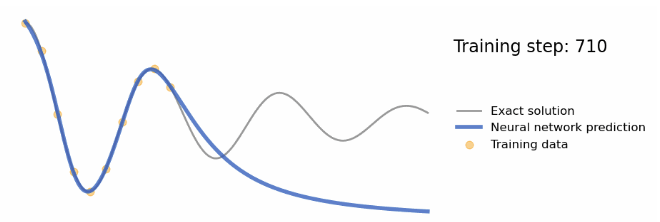
\includegraphics[width=0.75\textwidth]{img/redNeuronal01.png}
    \end{center}
        \begin{tablenotes}
            \item {{\fontsize{10pt}{ \baselineskip}\selectfont \textit{Nota.} Tomado de \url{https://benmoseley.blog/my-research/so-what-is-a-physics-informed-neural-network/} }}
        \end{tablenotes}
\end{figure}

Una forma popular de hacer esto usando el aprendizaje automático es usar una red neuronal. Dada la ubicación de un punto de datos como entrada (indicado como x), se puede usar una red neuronal para generar una predicción de su valor (indicado tucomo ), como se muestra en la figura \ref{figure:redNeuronal02}:
\begin{figure}[htbp]
    \caption{Esquema de una red neuronal\sep}
    \label{figure:redNeuronal02}
    \begin{center}
        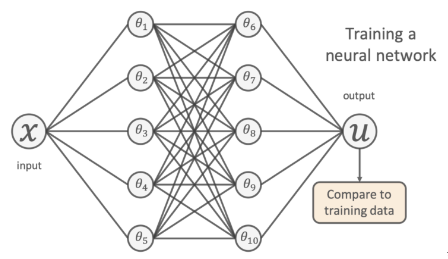
\includegraphics[width=0.75\textwidth]{img/redNeuronal02.png}
    \end{center}
        \begin{tablenotes}
            \item {{\fontsize{10pt}{ \baselineskip}\selectfont \textit{Nota.} Tomado de \url{https://benmoseley.blog/my-research/so-what-is-a-physics-informed-neural-network/}}}
        \end{tablenotes}
\end{figure}

Para aprender un modelo, tratamos de ajustar los parámetros libres de la red (indicados por la \ thetas en la figura anterior) para que las predicciones de la red coincidan estrechamente con los datos experimentales disponibles. Esto generalmente se hace minimizando el error cuadrático medio entre sus predicciones y los puntos de entrenamiento;
\begin{equation}
    min \frac{1}{N} \sum^N_i \left(u_{NN}(x_i;\theta) - u_{true}(x_i)\right)^2
\end{equation}
En la figure \ref{figure:redNeuronal01} se muestra el resultado de entrenar una red neuronal de este tipo utilizando los datos experimentales anteriores.

El problema es que usar un enfoque puramente basado en datos como este puede tener desventajas significativas. Eche un vistazo a los valores reales del proceso físico desconocido utilizado para generar los datos experimentales en la figura \ref{figure:redNeuronal01} (línea gris).

Puede ver que, si bien la red neuronal modela con precisión el proceso físico en la vecindad de los datos experimentales, no logra generalizar a partir de estos datos de entrenamiento. Confiando únicamente en los datos, se podría argumentar que realmente no ha “comprendido” el problema científico.

Si quisieramos solucionar el siguiente problema físico:
\begin{equation}
    m \frac{d^2 u}{d x^2} + u\frac{du}{dx} + ku = 0
\end{equation}
Donde $m$ es la masa del oscilador, $\mu$ es el coeficiente de fricción y $k$ es la constante del resorte.

Al usar el esquema de RN de la figura \ref{figure:digrama de flujo PINN} podemos ver que la pérdida física adicional en la función de pérdida intenta asegurar  que la solución aprendida por la red sea consistente con la física conocida, mediante la siguiente función de pérdida para entrenar la red.
\begin{equation}
    min \frac{1}{N}\sum^N_i \left(u_{NN}()x_i; \theta) - u_{true}(x_i)\right)^2 + \frac{1}{M}\sum^M_j\left(\left[m\frac{d^2}{dx^2}+\mu\frac{d}{dx}+k\right]u_{NN}(x_j;\theta)\right)^2
\end{equation}

\begin{figure}[htbp]
    \caption{Diagrama de flujo del algoritmo PINN\sep}
    \label{figure:digrama de flujo PINN}
    \begin{center}
        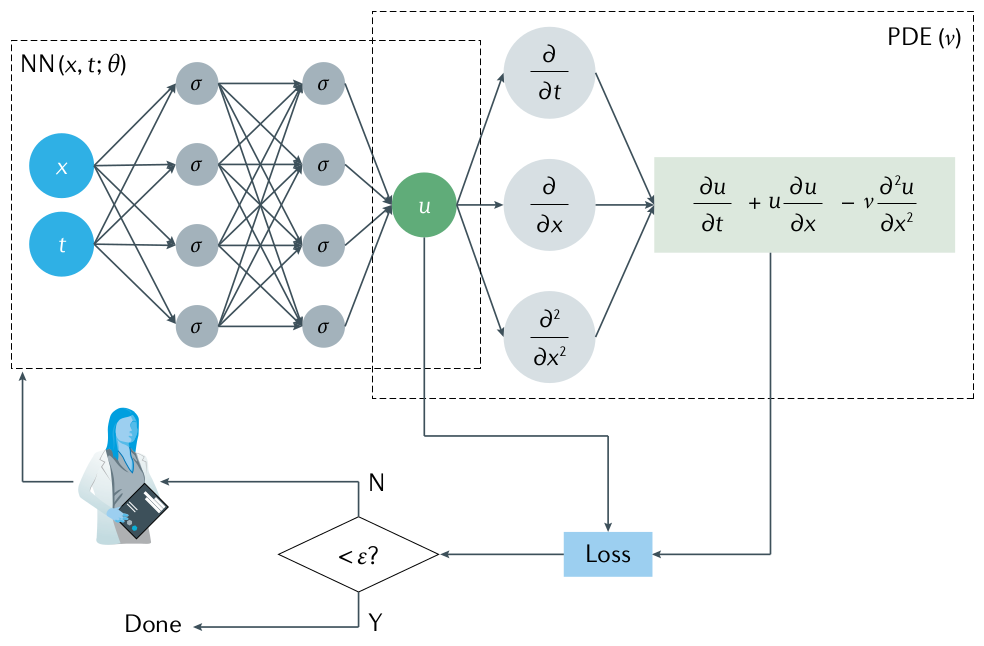
\includegraphics[width=0.75\textwidth]{img/pinns01.png}
    \end{center}
        \begin{tablenotes}
            \item {{\fontsize{10pt}{ \baselineskip}\selectfont \textit{Nota.} Tomado de ``Physics-informed machine learning'' (p. 425), por \citeauthor{Karniadakis2021}, \citeyear{Karniadakis2021}, \textit{Nature Reviews Physics, 3.} }}
        \end{tablenotes}
\end{figure}
Los resultados cuando entrenamos la red informada por la física podemos verlo en la figura \ref{figure:redNeuronal03}
\begin{figure}[htbp]
    \caption{Red neuronal informada por la física que aprende a modelar un oscilador armónico\sep}
    \label{figure:redNeuronal03}
    \begin{center}
        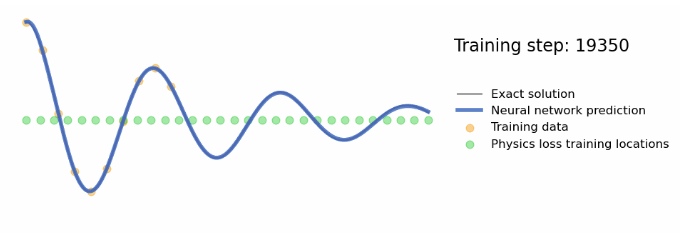
\includegraphics[width=0.75\textwidth]{img/redNeuronal03.png}
    \end{center}
        \begin{tablenotes}
            \item {{\fontsize{10pt}{ \baselineskip}\selectfont \textit{Nota.} Tomado de \url{https://benmoseley.blog/my-research/so-what-is-a-physics-informed-neural-network/}}}
        \end{tablenotes}
\end{figure}

% \section{Ecuación de onda}
% \subsection{La ecuación de onda y sus caracterísiticas}
% \subsection{Solución numérica de la ecuación de onda y sus características}


% \section{Construcción de una red neuronal informada por la física}




% La redes neuronales (RN) son la unidad funcional del aprendizaje profundo que imita el comportamiento del cerebro humano para resolver problemas complejos basados en datos. Los datos de entradas se procesan a través de diferentes capas de neuronas artificiales apiladas para producir el resultado deseado. Diversas investigaciones(\cite{Breen2019}; \cite{Raissi2017}; \cite{Nguyen2021}; \cite{Scellier2021}; \cite{Iten2018}) .

% Las entradas, que vienen a ser los {\it features}, ingresan al cuerpo de la ''neurona`` multiplicandose cada uno por unos pesos, realizando una combinación lineal de los pesos con los {\it features} $u_i = \sum_j = w_{ij} y_j$. Seguidamente se define una función $y_i = f(u_i)$, la cual tiene que garantizar la no linealidad.





% \begin{figure}[htbp]
%     \caption{Red neurona artificial y biológica\sep}
%     \label{fig:red neuronal y biologica}
%     \begin{center}
%         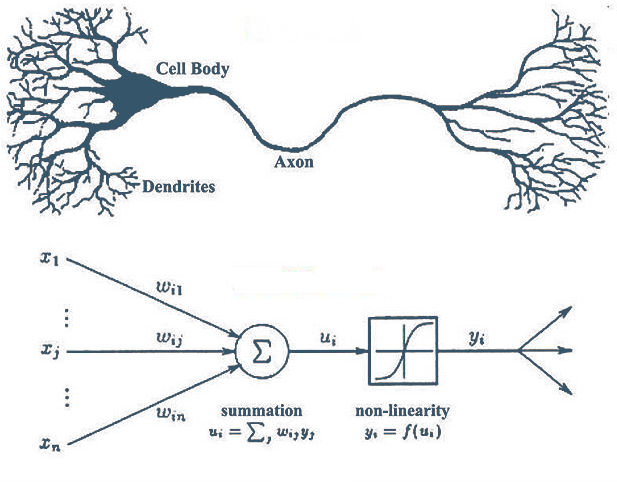
\includegraphics[width=0.6\textwidth]{img/red_neuronal.png}
%     \end{center}
%         % \begin{tablenotes}
%         %     \item {{\fontsize{10pt}{ \baselineskip}\selectfont \textit{Nota.} }}
%         % \end{tablenotes}
% \end{figure}

% 
% \section{Objetivos generales}
% Caracterizar los recursos hídricos e identificar las zonas vulnerables en el ámbito del Proyecto Especial Tambo Ccaracocha mediante el modelamiento geoespacial y presentar alternativas de aprovechamiento de los recursos hídricos.

% \section{Objetivos específicos}
% % [leftmargin=1em]
% \begin{itemize}
%     \item Determinar la oferta y demanda hídrica en el ámbito de influencia del Proyecto Especial Tambo-Ccaracocha. 
%     \item Presentar alternativas de proyectos, para contribuir a la segurar el afianzamiento hídrico para el valle de Ica. 
%     \item Generar una base de datos geoespacial, para caracterizar e identificar el grado de vulnerabilidad en el ámbito del Proyecto Tambo Ccaracocha.
%     \item Desarrollar el modelo geoespacial para identificación del grado de vulnerabilidad en el ámbito del Proyecto. 
% \end{itemize}



\chapter{Método}
\thispagestyle{empty}

\section{Tipo de investigación}
% SECTION - 
% * Su propósito es: Responder preguntas de investigación, Cumplir objetivos del estudio, Someter hipótesis a prueba.

% NOTE - 
% * Tipo Experimental: porque se puede controlar las variables.
% * Tipo longitudinal: 
% * Tipo analítico:
% * Tipo prospectivo.

La investigación es de tipo experimental, porque se puede medir la precisión y la perdida de las salidas de las redes neuronales. Tenemos control sobre la modificación de la variable independiente, parámetro de la RN. Tambíen es de tipo analítica, analizando las causas  del desempeño de la red frente a la solución de la EDP de la onda.



\section{Ámbito temporal y espacial}


\section{Variables}
% SECTION 
% * Las variables deben ser: comprensibles, precisos y concretos. 
% * La RELACIÓN entre variables debe ser: clara y verosímil. 
% * Observables y medibles, así como la relación planteada.
% * Deben estar relacionadas con técnicas disponibles para probarlas. (Curva ROC, precisión por épocas, la pérdida.)
%  * Generalmente surgen de los objetivos.

% NOTE - Según: 
% * Su naturaleza.- Cuantitativa: la exactitud y la perdida se expresan numéricamente. Variables continua.
% * A su dominio.- V. Independiente: parámtros de la red, función de perdida. V. Dependiente: Valores de la solución estraploada. 
% * Su amplitud.- None
% * Su nivel de abstracción.- V. Empirica: Los errores y la perdida se pueden medir con instrumentos estadísticos.
% * Carácter de las escalas o por su calor de medición.- Variable cardinal; variable de intervalo, Curva ROC.
% * Grado de complejidad.- Simple, una dimensión; Desempeño de la red neuronal.

\begin{itemize}
    \item Según su naturaleza.-
    La variable es cuantitativa, sabiendo que la exactitud y la pérdida se expresan numéricamente, considerandose, de la misma forma variables continuas.

    \item Según su dominio
    \begin{itemize}
        \item Variable Independiente.- Los parámetrod de la red y la función de perdida acotada con la Ecuación Diferencial de Onda.
        \item Variable Dependiente.- Valores de la solución extrapolada.
    \end{itemize}

    \item Según su nivel de abstracción.- 
    Variable Empirica, Los errores y la pérdida se pueden medir con instrumentos estadísticos.

    \item Según el carácter de las escalas.-
    Variable cardinal.

    \item Según el grado de complejidad.-
    Simple, El desempeño de la red neuronal.
\end{itemize}

\section{Población y muestra}
\section{Instrumentos}
\section{Procedimientos}
\section{Análisis de datos}
\section{Consideraciones éticas (si fuera necesario)}

% \begin{figure}[htbp!]
%     \caption{UNFV\sep}
%     \label{fig:1}
%     \begin{center}
%         
\includegraphics[width=0.3\textwidth]{Cover/UNFV.png}
%     \end{center}
%     \begin{tablenotes}
%         \item {{\fontsize{10pt}{ \baselineskip}\selectfont \textit{Nota.} Elaboración propia}}
%     \end{tablenotes}
% \end{figure}

% Al aplicar el modelo SEBAL, es importante la selección de dos píxeles ``ancla'' (píxel ``caliente" y ``frío") sobre el área de interés, que se utilizan para determinar las diferencias de temperatura entre la temperatura de la superficie ($T_{s}$) y la temperatura del aire ($dT$). Se supone que existe una relación lineal entre $T_{s}$ y $dT$ en forma de:
% \begin{equation}
%     dT = aT_{s} + b
% \end{equation}
% donde a y b son las constantes de relación lineal. Para determinar estas constantes, SEBAL utiliza los dos píxeles ``ancla" para los cuales se puede estimar confiablemente un valor para h. $T_{s}$ se estima a partir de la temperatura de la superficie terrestre (LST)  para cada píxel; $dT$ se calcula para el píxel ``caliente" o ``frío" utilizando la siguiente relación:
% \begin{equation}
%     dT_{\frac{cold}{hot}} = h_{\frac{cold}{hot}}{r_{ah}}_{\frac{cold}{hot}}/\left ( \rho_{\frac{cold}{hot}}c_{p} \right )
% \end{equation}
% donde h puede calcularse para los píxeles de anclaje utilizando datos meteorológicos, $\rho$  es la densidad del aire ($kg\times m^{-3}$), $Cp$ es el calor específico del aire ($1004 J\times kgK^{-1}$), $dT$ es la diferencia de temperatura entre dos alturas ($K$), y rah es la resistencia aerodinámica al transporte de calor ($s\times m^{-1}$) para cada píxel ``frío" y ``caliente". La anterior relación lineal entre $dT$ y $T_{s}$ es una presunción importante en el SEBAL.

% El píxel frío se utiliza para definir la cantidad de evapotranspiración. Para identificar los píxeles fríos en la zona de interés se suele utilizar un cultivo o una masa de agua que cubra toda la superficie. Sin embargo, la temperatura de la superficie que se utiliza debe ajustarse uniformemente a una elevación de referencia común para una predicción precisa de $dT$. De lo contrario, las altas elevaciones que parecen ``frías" pueden interpretarse erróneamente como que tienen una alta evaporación. Por ello se procede a realizar una corrección de la temperatura. En el procedimiento se utilizaron los datos del MED para este cálculo. La temperatura superficial corregida por el MED es calculada por la siguiente ecuación:
% \begin{equation}
%     T_{0_{-}dem} = T_{0} + 0.0065\Delta z
% \end{equation}
% donde $\Delta z $ es la diferencia de la elevación de un píxel con respecto al dato ($m$).

% A partir del residuo en la ecuación de balance energético instantáneo y la fracción de evaporación ($\Lambda$), se estimó el ET diario ($ET_24$), $mm\times d^{-1}$. $\Lambda$ es notablemente regular y relativamente constante en los días sin nubes. Por lo tanto, su valor instantáneo puede tomarse como el valor medio diario, de modo que la variabilidad espacial en la ET diaria puede predecirse a gran escala.
% \begin{equation}
%     \Lambda = \frac{\lambda ET}{R_{n} - G}
% \end{equation}
% \begin{equation}
%     ET_{24} = \frac{86500\Lambda \left ( R_{n,24} - G_{24} \right )}{\lambda }
% \end{equation}
% donde $R_{n,24}$ es la radiación neta diaria; $G_{24}$ es el flujo de calor diario del suelo; 86.400 es el número de segundos en un período de 24 h; y $\Lambda$ es el calor latente de vaporización ($J\times kg^{-1}$). El calor latente de vaporización permite la expresión de $ET_{24}$ en $mm\times d^{-1}$. El parámetro $G_{24}$ puede ser aproximado para las superficies vegetativas y del suelo como cero en la superficie del suelo. Esto se debe a que, en promedio, la energía almacenada en el suelo durante el día se libera en el aire durante la noche. La vaporización de calor latente y $R_{n,24}$ se definen como:
% \begin{gather}
%      \lambda = \left ( 2.501 - 0.00236\left ( T_{0} - 273 \right )\times 10^{6}  \right ) \left (  J\times kg^{-1}\right ) \\
%      R_{n,24} = \left ( 1 - \alpha  \right )Rs_{24} - a\tau _{sw}
% \end{gather}
% donde $Rs_{24}$ es la radiación solar entrante de 24 horas; alfa es el albedo; a es un coeficiente de regresión de la relación entre la radiación de onda larga neta y la transmisibilidad atmosférica a escala diaria; y $\tau _{sw}$ es la de transmisión unidireccional en un cielo claro y puede predecirse para condiciones atmosféricas claras y relativamente secas utilizando la elevación sobre el nivel del mar en $m$. El coeficiente a puede aplicarse de manera diferente según a la región.

% \parencite{Lee2016} estimaron la evapotranspiración espacial diaria utilizando el algoritmo SEBAL modificado con una selección automática mejorada para el píxel de ancla y datos mensuales para mejorar los resultados, utilizando los datos del Terra MODIS para Corea del Sur. Los mismos que constan de  36 canales espectrales discretos con una resolución espacial de 250 m para bandas visibles, 500 m para bandas de infrarrojo cercano y 1000 m para las bandas de infrarrojos térmicos restantes. Los resultados espaciales de la ET obtenidos mediante el modelo SEBAL se validaron utilizando dos años (2012-2013) de datos de ET de torres de flujo medidos en tres lugares (dos en un bosque y uno en un arrozal). 

% Para píxeles\footnote{Medida de cada cuadrante del espectro.} fríos, se selecciono el 5\% superior del NDVI más alto y, entre ellos, se selecciono el 15\% más frío de la Ts dentro de un área agrícola del área según el uso de la tierra. Para píxeles calientes, se selecciono el 10\% más bajo del NDVI y luego se selecciono el 15\% más caliente de la Ts dentro de un campo desnudo o un área urbana de acuerdo con el uso de la tierra. Se hace referencia al estándar para los candidatos a píxeles de anclaje, sin embargo, el porcentaje se ajusta ligeramente de 20\% a 15\% porque hay muchos píxeles en el área de interés y puede afectar el tiempo de ejecución total del modelo. Durante el período de este estudio (2012-2013), el valor máximo de la temperatura superficial de la tierra (LST) mostró el rango de aproximadamente 279.2 K a 321.0 K, mientras que el valor mínimo de LST indicó el rango de aproximadamente 252,1 K a 295,4 K. Generalmente, los píxeles calientes se seleccionaron en el rango de 277,1 K a 319,1 K, y los píxeles fríos se incluyeron en el rango de 253,6 K a 296,4 K. El LST fue el factor clave, además de los datos de los satélites, para estimar la variabilidad temporal diaria de la ET \parencite{Lee2016}.

% \lipsum[1]

% \lipsum[3]

% \begin{table}[H]
% \centering
% \begin{threeparttable}
% \caption{Características de la torre de flujo CFK ubicada al centro de arrozales}
% \label{tab:1}
% \begin{tabular}{@{}lc@{}}
% \hline
% \multicolumn{1}{c}{Sitio} & Cheongmicheon (CFK) \\ \hline
% Latitud (N) & 37$^{\circ}$ 090 35” \\
% Longitud (E) & 127$^{\circ}$ 390 10” \\
% Elevación (m) & 141 \\
% Temperatura media anual ($^{\circ}$C) & 11.5 \\
% Precipitación media anual (mm) & 1107 \\
% Velocidad del viento media (m/s) & 1.97 \\
% Tierra usada & Arrozal \\ \hline
% \end{tabular}
%     \begin{tablenotes}
%     \vspace{-0.5cm}
%       \item {{\fontsize{10pt}{ \baselineskip}\selectfont \textbf{FUENTE}: \parencite{Lee2016}}}
%     \end{tablenotes}
% \end{threeparttable}
% \end{table}
% \vspace{-0.6cm}
% La Figura \ref{fig:2} muestra la variación diurna de los componentes de balance energético sobre la superficie transpirante bien regado en un día despejado en un arrozal. El flujo de calor del suelo se encuentra en el rango de 0 a 100 $W\times m^{-2}$ y el flujo de calor sensible se encuentra en el rango de aproximadamente 50 a 400 $W\times m^{-2}$.

% \begin{figure}[H]
%     \centering
%     \includegraphics[width=0.4\textwidth]{Cover/Escudo_UNALM.pdf}
%     \caption{Variación temporal de los componentes del balance energético en la torre de flujo ubicada al centro de arrozales}
%     \captionsetup{labelfont=rm,skip=2pt,textfont=rm,font=small}
%         \caption*{\textbf{FUENTE:} \parencite{Lee2016}}
%     \label{fig:2}
% \end{figure}

% En condiciones climáticas casi nubladas, la radiación solar ($Rs$) en lugar de $Ra(24)t(sw)$, mejoró los resultados del r2 del SEBAL en arrozales de 0,52 a 0,77, es decir se debe utilizar un valor medido local (en tierra) para la radiación solar (Rs) de 24 horas en lugar de $Ra(24)\tau (sw)$. Esto depende del porcentaje de nubosidad del lugar de estudio. Ver Figura \ref{fig:3}. 

% \begin{figure}[H]
%     \centering
%     \includegraphics[width=0.3\textwidth]{Cover/Escudo_UNALM.pdf}
%     \caption{UNALM}
%     \captionsetup{labelfont=rm,skip=2pt,textfont=rm,font=small}
%         \caption*{\textbf{FUENTE:} \parencite{Lee2016}}
%     \label{fig:3}
% \end{figure}
% \vspace{-0.6cm}
% La Figura \ref{fig:4} se muestra la ET en arrozales obtenida por \parencite{Lee2016} con ET total de 496,1 y 467,8 mm para el 2012 y 2013 respectivamente (torre de flujo) y 5,2 y 5,3 $mm\times d^{-1}$ según la torre de flujo y SEBAL, respectivamente; con mejor ajuste de la ET para el año 2013 con valores de Indice de Nash de 0.73 y r2 de 0.80.

% \begin{figure}[H]
%     \centering
%     \includegraphics[width=0.4\textwidth]{Cover/Escudo_UNALM.pdf}
%     \caption{UNALM}
%     \captionsetup{labelfont=rm,skip=2pt,textfont=rm,font=small}
%         \caption*{\textbf{FUENTE:} \parencite{Lee2016}}
%     \label{fig:4}
% \end{figure}
% \vspace{-0.6cm}
% La Figura \ref{fig:5} muestra los datos mensuales del NDVI, el albedo y  ET según las torres de flujo. El NDVI de la zona de arrozales muestra el patrón de crecimiento y desarrollo de la planta de mayo a septiembre, el NDVI de las zonas de bosques mixtos muestra un patrón diferente, con valor superior a 0,5 de abril a noviembre. En la temporada de invierno (particularmente en diciembre), el NDVI del bosque tiende a ser más bajo que el de arrozales, esto debido a que está situado a una mayor altitud. Es decir, SEBAL refleja las características geográficas, con  ET en las zonas bajas, mayores que en zonas de mayor altitud.

% \begin{figure}[H]
%     \centering
%     \includegraphics[width=0.4\textwidth]{Cover/Escudo_UNALM.pdf}
%     \caption{UNALM}
%     \captionsetup{labelfont=rm,skip=2pt,textfont=rm,font=small}
%         \caption*{\textbf{FUENTE:} \parencite{Lee2016}}
%     \label{fig:5}
% \end{figure}
% \vspace{-0.6cm}
% \lipsum[3]

% \lipsum[2]

% \subsection{METRIC}

% \lipsum[1]

% \lipsum[2]

% \parencite{Bhattarai2017} estimaron la ET en tres sitios del USA con sitios de flujo EC en FL y un sitio llamado Ameriflux, Medición de la Radiación Atmosférica en las Grandes Llanuras del Sur (ARM SGP), en OKLAHOMA (OK), informacion que se utilizaron para demostrar el modelo automatizado desarrollado en este estudio.  La estación de Blue Cypress cubre un gran sistema de humedales de llanura de inundación en la cabecera del río St. Johns en el condado de Indian River en el centro-oeste. El sitio de Citrus cubre una arboleda de 22 ha de cítricos de bosque plano. La Ferris está situado en zona de pastos (Paspalum notatum) y los campos de fresas. El sitio ARM-SGP es una gran estación agrícola experimental (periódica rotación del trigo, el maíz y la soja) con un clima más seco.

% \subsubsection{Los datos medidos de la ET}

% \lipsum[4]

% \begin{table}[H]
% \centering
% \begin{threeparttable}
% \caption{Descripción de los sitios utilizados en este estudio}
% \label{tab:2}
% \begin{tabular}{@{}lc@{}}
% \hline
% \multicolumn{1}{c}{Descripciones del sitio} & ARM SGP \\ \hline
% Latitud ($^{\circ}$N) & 36.6058 \\
% Longitud ($^{\circ}$W) & 97.4888 \\
% Tipo de cobertura & Cultivos \\
% Periodo de medición de la ET$^{a}$ & 2000-2015 \\
% Tiempo medio anual ($^{\circ}$C) & 15 \\
% Precipitación media anual (mm) & 383 \\
% La media diaria de la ET (mm dia) & 1.3 \\
% Altura del dosel (m) & Variante \\
% Altura de la torre (m) & 60 \\
% Fuente para más información & ARM Climate Research Facility \\ \hline
% \end{tabular}
%     \begin{tablenotes}
%     \vspace{-0.5cm}
%       \item {{\fontsize{10pt}{ \baselineskip}\selectfont \textbf{FUENTE}: \parencite{Bhattarai2017}}}
%     \end{tablenotes}
% \end{threeparttable}
% \end{table}
% \vspace{-0.6cm}
% Diseñamos específicamente nuestro algoritmo de automatización para trabajar con imágenes térmicas de Landsat. El tamaño de 30 m de píxeles - la banda térmica es remuestreada a 30 m para igualar las bandas multiespectrales. Landsat permite el mapeo de la ET a escalas de campo, por lo que los datos de Landsat son ampliamente utilizados en la gestión de los recursos hídricos.  Las imágenes Landsat de La superficie se procesaron por el Sistema de Procesamiento Adaptativo de Perturbaciones (LEDAPS) reflectancia (Masek et al., 2006) (bandas 1-5 y 7), la imagen termal Landsat y los metadatos de la imagen se obtuvieron del USGS (\url{www.glovis.usgs.gov} y \url{http://landsat.usgs.gov/lsrd_sw.php}; último acceso 06/10/2015). Las ortoimágenes a nivel estatal con un tamaño de 1 m de píxel se obtuvieron del Departamento de Agricultura de los Estados Unidos (USDA).

% \subsubsection{Las datos Meteorológicos}

% Datos meteorológicos de intervalo temporal de 15 minutos disponibles gratuitamente desde la plataforma de la Red Meteorológica Automatizada de la Florida (FAWN) (Figura 6; \url{http://fawn.ifas.ufl.edu/ about_index.php} y Oklahoma Mesonet  \url{https://www.mesonet.org/} se utilizaron en este estudio. Un mapa ráster para cada estación instantánea y los parámetros meteorológicos diarios (es decir, velocidad del viento, temperatura, la radiación solar, y la humedad relativa).

% \subsubsection{Datos de la Cubierta Terrestre}

% Datos disponibles de 30 m de cobertura terrestre del USGS National Land Cover Base de datos (NLCD; \url{http://www.mrlc.gov/index.php}) se utilizaron para identificar las tierras agrícolas tanto para el manual como para  los enfoques automatizados de selección de píxeles de los miembros.  Las tierras agrícolas incluían ambos cultivos y los pastos. Las descripciones e implementación de los modelos SEBAL y MÉTRIC, se basan en que la ET puede ser estimada a partir del término residual del balance energético de la superficie ecuación (Ec. (1)). Rn se calcula para las condiciones de cielo despejado (Ec. (9)) G se calcula como la fracción de Rn (Ec. (10)).

% \begin{table}[H]
% \centering
% \begin{threeparttable}
% \caption[Estaciones meteorológicas]{\textbf{Estaciones meteorológicas}}
% \label{tab:my-tablez}
% \begin{tabular}{@{}lcccc@{}}
% \hline
% Estaciones & Este (m) & Norte (m) & Latitud & Longitud \\ \hline
% Tunel cero & 490680.81 & 8534186.15 & 13$^{\circ}$15'33.54'' & 75$^{\circ}$5'8'' \\
% Ocucaje & 426464.86 & 8410316.41 & 14$^{\circ}$22'42.2'' & 75$^{\circ}$40'0'' \\ \hline
% \end{tabular}
%     \begin{tablenotes}
%     \vspace{-0.5cm}
%       \item {{\fontsize{10pt}{ \baselineskip}\selectfont \textbf{FUENTE}: Elaboración propia}}
%     \end{tablenotes}
% \end{threeparttable}
% \end{table}

% \newpage
% \begin{landscape}
% \pagestyle{empty}
% \begin{figure}
%     \centering
%     \includegraphics[width=1\textwidth]{Figures/f2.png}
%     \caption{Diagrama de modelos}
%     \label{fig:my_label5}
% \end{figure}
% \end{landscape}




\chapter{Aspectos administrativos}
\thispagestyle{empty}

\section{Cronograma de actividades}
\section{Presupuesto}
\section{Fuentes de financiamiento}

% \begin{itemize}[leftmargin=1em]
%     \item La siguiente Tabla \ref{tab:my-table1} es de clasificación de suelos:
% \end{itemize}
% \begin{table}[H]
% \centering
% \begin{threeparttable}
% \caption[Clasificación de suelos]{Clasificación de suelos para determinarlo en el laboratorio del departamento de ordenamiento territorial}
% \label{tab:my-table1}
% \begin{tabular}{@{}ccccc@{}}
% \hline
% \multicolumn{1}{|c|}{} &
%   \multicolumn{1}{c|}{BRITÁNICO} &
%   \multicolumn{1}{c|}{AASHTO} &
%   \multicolumn{1}{c|}{ASTM} &
%   \multicolumn{1}{c|}{SUCS} \\ \cline{2-5} 
% \multicolumn{1}{|c|}{\multirow{-2}{*}{SISTEMAS}} &
%   \multicolumn{1}{c|}{{\color[HTML]{4D5156} (mm)}} &
%   \multicolumn{1}{c|}{{\color[HTML]{4D5156} (mm)}} &
%   \multicolumn{1}{c|}{{\color[HTML]{4D5156} (mm)}} &
%   \multicolumn{1}{c|}{{\color[HTML]{4D5156} (mm)}} \\ \hline
% \multicolumn{1}{|c|}{Grava} &
%   \multicolumn{1}{c|}{60 - 2} &
%   \multicolumn{1}{c|}{75 - 2} &
%   \multicolumn{1}{c|}{\textgreater 2} &
%   \multicolumn{1}{c|}{75 - 4,75} \\ \hline
% \multicolumn{1}{|c|}{Arena} &
%   \multicolumn{1}{c|}{2 - 0,006} &
%   \multicolumn{1}{c|}{2 - 0,05} &
%   \multicolumn{1}{c|}{2 - 0,075} &
%   \multicolumn{1}{c|}{4,75 - 0,075} \\ \hline
% \multicolumn{1}{|c|}{Limo} &
%   \multicolumn{1}{c|}{0,06 - 0,002} &
%   \multicolumn{1}{c|}{0,05 - 0,002} &
%   \multicolumn{1}{c|}{0,075 - 0,005} &
%   \multicolumn{1}{c|}{\textless 0,075 FINOS} \\ \hline
% \multicolumn{1}{|c|}{Arcilla} &
%   \multicolumn{1}{c|}{\textless  0,002} &
%   \multicolumn{1}{c|}{\textless  0,002} &
%   \multicolumn{1}{c|}{\textless  0,005} &
%   \multicolumn{1}{c|}{} \\ \hline
% \end{tabular}
%     \begin{tablenotes}
%     \vspace{-0.5cm}
%       \item {{\fontsize{10pt}{ \baselineskip}\selectfont \textbf{FUENTE}: Elaboración propia}}
%     \end{tablenotes}
% \end{threeparttable}
% \end{table}


% \begin{table}[H]
%     \centering
%     \begin{threeparttable}
%         \caption{Estaciones meteorológicas \sep}
%         \label{tab:my-table}
%         \begin{tabular}{@{}lcccc@{}}
%             \hline
%             Estaciones & Este (m)  & Norte (m)  & Latitud                & Longitud           \\ \hline
%             Tunel cero & 490680.81 & 8534186.15 & 13$^{\circ}$15'33.54'' & 75$^{\circ}$5'8''  \\
%             Ocucaje    & 426464.86 & 8410316.41 & 14$^{\circ}$22'42.2''  & 75$^{\circ}$40'0'' \\ \hline
%         \end{tabular}
%         \begin{tablenotes}
%             \item {{\fontsize{10pt}{ \baselineskip}\selectfont \textit{Nota.} Elaboración propia}}
%         \end{tablenotes}
%     \end{threeparttable}
% \end{table}

% \begin{table}[H]
% \centering
%   \begin{threeparttable}
% \caption{Estaciones meteorológicas}
% \label{tab:my-table2}
% \begin{tabular}{@{}lcccc@{}}
% \hline
% Estaciones & Este (m) & Norte (m) & Latitud & Longitud \\ \hline
% Tunel cero & 490680.81 & 8534186.15 & 13$^{\circ}$15'33.54'' & 75$^{\circ}$5'8'' \\
% Ocucaje & 426464.86 & 8410316.41 & 14$^{\circ}$22'42.2'' & 75$^{\circ}$40'0'' \\ \hline
% \end{tabular}
%     \begin{tablenotes}
%     \vspace{-0.5cm}
%       \item {{\fontsize{10pt}{ \baselineskip}\selectfont \textbf{FUENTE}: Elaboración propia}}
%     \end{tablenotes}
% \end{threeparttable}
% \end{table}

% \begin{figure}[H]
%     \centering
%       \caption{Comparación entre Qdisponible y Qdemanda}
%         \includegraphics[width=0.7\textwidth]{Figures/Comparation.pdf}
%         \captionsetup{labelfont=rm,skip=2pt,textfont=rm,font=small}
%         \caption*{\textbf{FUENTE:} Elaboración propia}
%     \label{fig:12}
% \end{figure}

% \begin{itemize}
%     \item En la Figura \ref{fig:21}, se muestran los volúmenes medios mensuales acumulados de la estación Santa Eulalia (1972-1992).
% \end{itemize}

% \begin{figure}[H]
%     \centering
%     \includegraphics[width=0.7\textwidth]{Figures/Volumenes.pdf}
%     \caption{Volúmenes medios mensuales acumulados}
%     \captionsetup{labelfont=rm,skip=2pt,textfont=rm,font=small}
%         \caption*{\textbf{FUENTE:} Servicio Nacional de Meteorología e Hidrología del Perú SENAMHI}
%     \label{fig:21}
% \end{figure}

% \begin{table}[H]
% \centering
%   \begin{threeparttable}
%     \caption{Sample ANOVA table}
%      \begin{tabular}{lllll}
%         \toprule \toprule
%         Stubhead & \( df \) & \( f \) & \( \eta \) & \( p \) \\
%         \midrule
%                  &     \multicolumn{4}{c}{Spanning text}     \\
%         Row 1    & 1        & 0.67    & 0.55       & 0.41    \\
%         Row 2    & 2        & 0.02    & 0.01       & 0.39    \\
%         Row 3    & 3        & 0.15    & 0.33       & 0.34    \\
%         Row 4    & 4        & 1.00    & 0.76       & 0.54    \\
%         \bottomrule
%      \end{tabular}
%     \begin{tablenotes}
%     \vspace{-0.5cm}
%         \item {{\fontsize{10pt}{ \baselineskip}\selectfont \textbf{FUENTE}: Elaboración propia}}
%     \end{tablenotes}
% \end{threeparttable}
% \end{table}






%\chapter{RESULTADOS Y DISCUSIÓN}
\thispagestyle{empty}
\begin{itemize}
    \item \lipsum[2]
    \item \lipsum[3]
\end{itemize}




%\chapter{CONCLUSIONES}
\thispagestyle{empty}
\section{Funcionamiento de muros de contención}
\begin{itemize}[leftmargin=1em]
    \item \lipsum[1]
    \item \lipsum[2]
    \item \lipsum[3]
    \item \lipsum[4]
\end{itemize}

%\chapter[\hspace{0.2cm}RECOMENDACIONES]{RECOMENDACIONES}
\thispagestyle{empty}
\section{Funcionamiento de muros de contención}
\begin{itemize}[leftmargin=1em]
    \item \lipsum[3]
    \item \lipsum[2]
    \item \lipsum[5] \parencite{Niu2020}.
    \parencite{Niu2020} \parencite[see][p10]{Niu2020}\nptextcite{Niu2020} hola \textcite{Niu2020}
\end{itemize}





\printbibliography[title={V.\hspace{1em}Referencias}]
\addcontentsline{toc}{chapter}{V. \textbf{Referencias}}
\thispagestyle{empty}

\appendix
\setcounter{chapter}{5}
\renewcommand{\thechapter}{\Roman{chapter}.}
\setcounter{section}{5}% Reset numbering for sections
\renewcommand{\thesection}{\arabic{chapter}.\arabic{section}}% Adjust

\chapter[ Anexos]{Anexos}
\thispagestyle{empty}

\section*{Anexo 1: Mapas de la zona de estudio}\appcaption{Anexo 1: Mapas de la zona de estudio}
...(contents of appendix one)...

% \begin{figure}[htbp!]
%     \centering
%     \includegraphics[width=0.9\textwidth]{Figures/f2.png}
%     % \addto\captionsspanish{\renewcommand{\appendixname}{Anexo}}
%     \caption*{Anexo 1.1: Variación temporal de los componentes del balance energético en la torre de flujo ubicada al centro de arrozales}
%     \captionsetup{labelfont=rm,skip=2pt,textfont=rm,font=small}
%         \caption*{\textbf{FUENTE:} \parencite{Lee2016}}
%     \label{fig:a1}
% \end{figure}

\section*{Anexo 2: Mapas de la zona de estudio}\appcaption{Anexo 2: Mapas de la zona de estudio}

\section*{Anexo 3: Mapas de la zona de estudio}\appcaption{Anexo 3: Mapas de la zona de estudio}


\end{document}
